%% control_*.eps se generan con test_control_bajo_nivel.m en MATLAB.
\subsection{Control de bajo nivel}

\subsubsection{Funcionamiento del control interno del servo S3003}
El S3003 es un servomotor con el lazo de posición cerrado \emph{dentro de la carcasa}; desde el microcontrolador (ESP32-S3) solo se envía una señal PWM de 50 Hz ($T=20$ ms) cuyo ancho de pulso (nominalmente 1--2 ms, 1,5 ms en el centro) codifica el ángulo deseado $\theta_{ref}$. La figura~\ref{fig:s3003} muestra la cadena interna:
\begin{enumerate}
 \item \textbf{Medidor de ancho de pulso}: un circuito monoestable convierte el ancho del pulso de entrada en la referencia $\theta_{ref}$.
 \item \textbf{Potenciómetro}: acoplado al eje de salida, entrega la posición medida $\theta$ (realimentación negativa).
 \item \textbf{Amplificador de error con banda muerta}: compara referencia y medida; entrega una señal proporcional al error $e=\theta_{ref}-\theta$, que equivale a un controlador \textbf{proporcional} de ganancia $K_p$ con saturación. La banda muerta (del orden de pocos $\mu$s, $\approx 0{,}5^\circ$) evita el vibrado alrededor de la referencia, y es coherente con la resolución de 0,5$^\circ$ usada en el sensor modelado.
 \item \textbf{Puente H}: aplica al motor una tensión $V\in[-6,6]$ V de signo igual al del error.
 \item \textbf{Motor DC + reductora}: el motor (modelo de las ecuaciones (3)--(5)) mueve el eje a través de los engranajes, que multiplican el par y reducen la velocidad; el potenciómetro cierra el lazo.
\end{enumerate}
En consecuencia, el servo se comporta como un lazo P de posición: para errores grandes el driver satura ($V=\pm6$ V, $\omega\approx\omega_{nl}=5{,}51$ rad/s, $i\le i_{stall}$) y para errores pequeños la velocidad es proporcional al error, sin sobreimpulso apreciable. No hay acción integral ni prealimentación, y el usuario no puede ajustar $K_p$.

\begin{figure}[h]\centering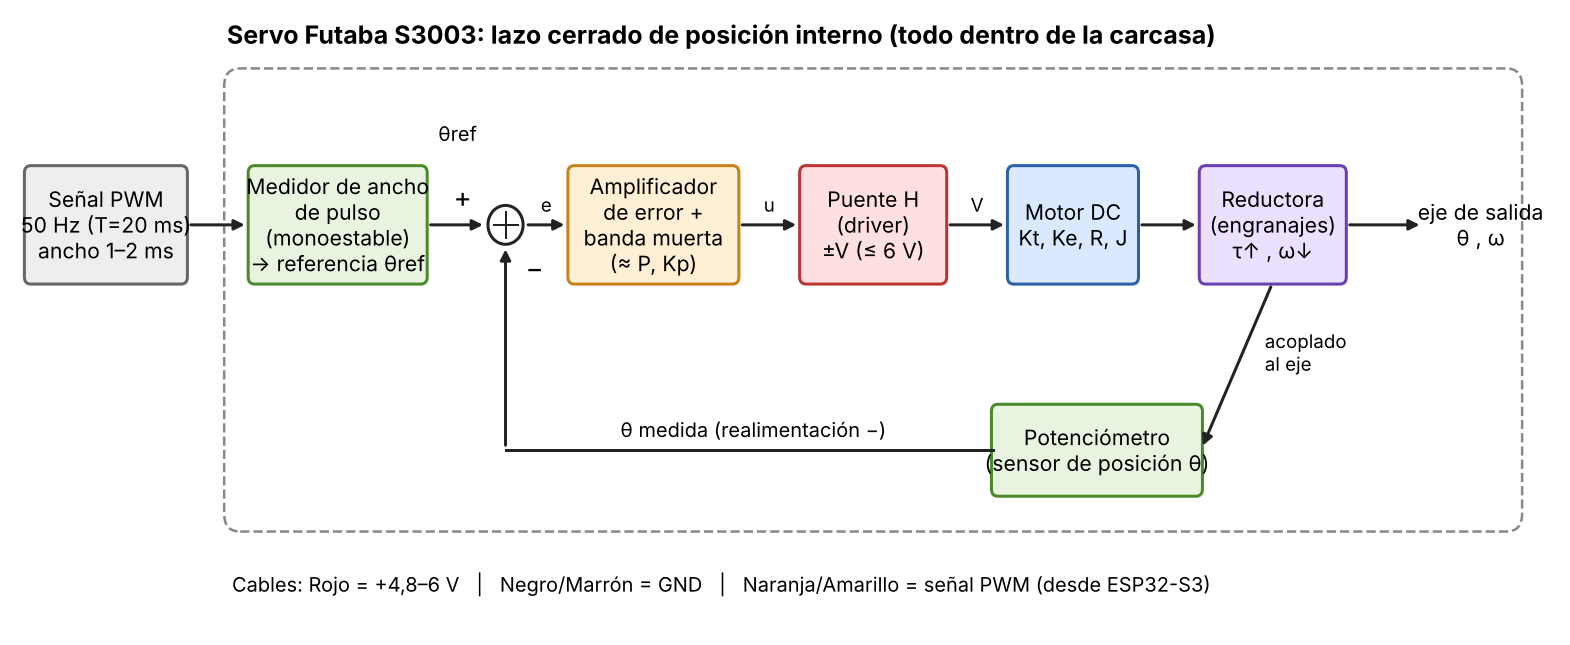
\includegraphics[width=\textwidth]{figuras/diag_s3003_interno.png}
\caption{Diagrama de bloques del control interno del servo Futaba S3003.}\label{fig:s3003}\end{figure}

\subsubsection{Diseño del control de bajo nivel (modelo en Simulink)}
Para simular el comportamiento de cada articulación se incluyó en cada instancia (\texttt{Joint1}, \texttt{Joint2}) el lazo de posición del servo, implementado con bloques base de Simulink (figura~\ref{fig:lazo}). La ley de control, evaluada cada $T_s=10$ ms con la posición \emph{medida} (cuantizada a 0,5$^\circ$, ruido de 0,05$^\circ$, saturada a $\pm90^\circ$), es
\begin{equation}
V_k=\mathrm{sat}_{\pm V_{max}}\!\left[K_p\big(\theta_{ref,k}-\theta_{med,k}\big)+K_e\,\dot\theta_{ref,k}\right],\qquad V_{max}=6\ \mathrm{V}.
\end{equation}
El primer término emula el lazo P del servo; el segundo es una prealimentación de velocidad (compensa la f.e.m., $V=K_e\omega$) que reduce el error de seguimiento en rampa y está disponible porque la cinemática inversa entrega $\dot q$.

\textbf{Sintonía.} Con $L=B=0$ la planta es $\theta/V=K/[s(\tau_m s+1)]$ con $K=0{,}9186$ rad/s/V y $\tau_m=4{,}11$ ms. En lazo cerrado con $K_p$ resulta $\tau_m s^2+s+KK_p=0$, con $\omega_n=\sqrt{KK_p/\tau_m}$ y $\zeta=1/(2\sqrt{KK_p\tau_m})$. Se eligió $KK_p=40$ s$^{-1}$, es decir
\begin{equation}
K_p=\frac{40}{K}=43{,}5\ \mathrm{V/rad}\;(0{,}76\ \mathrm{V/^\circ}),\qquad \zeta=1{,}23,\quad \omega_n=98{,}6\ \mathrm{rad/s}.
\end{equation}
Con el retardo del retenedor ($T_s/2$) el lazo abierto tiene $\omega_c=39{,}5$ rad/s, margen de fase de $69{,}5^\circ$ y margen de ganancia de 15,2 dB (figura~\ref{fig:bode}). El ancho de banda ($\approx 6$ Hz) es mucho mayor que el contenido espectral de las trayectorias de dibujo, pero suficientemente bajo para no amplificar la cuantización del sensor. No se incluyó acción integral: con la carga máxima (0,177 mN$\cdot$m) el error estático es $R\tau/(K_tK_p)\approx 6\times10^{-5}$ rad, muy por debajo de la resolución del sensor, y un integrador con cuantización de 0,5$^\circ$ provocaría ciclos límite. La corriente medida se registra para supervisión; como $V\le6$ V, la corriente queda acotada por $i_{stall}=0{,}3693$ A sin necesidad de un lazo de corriente.

\begin{figure}[h]\centering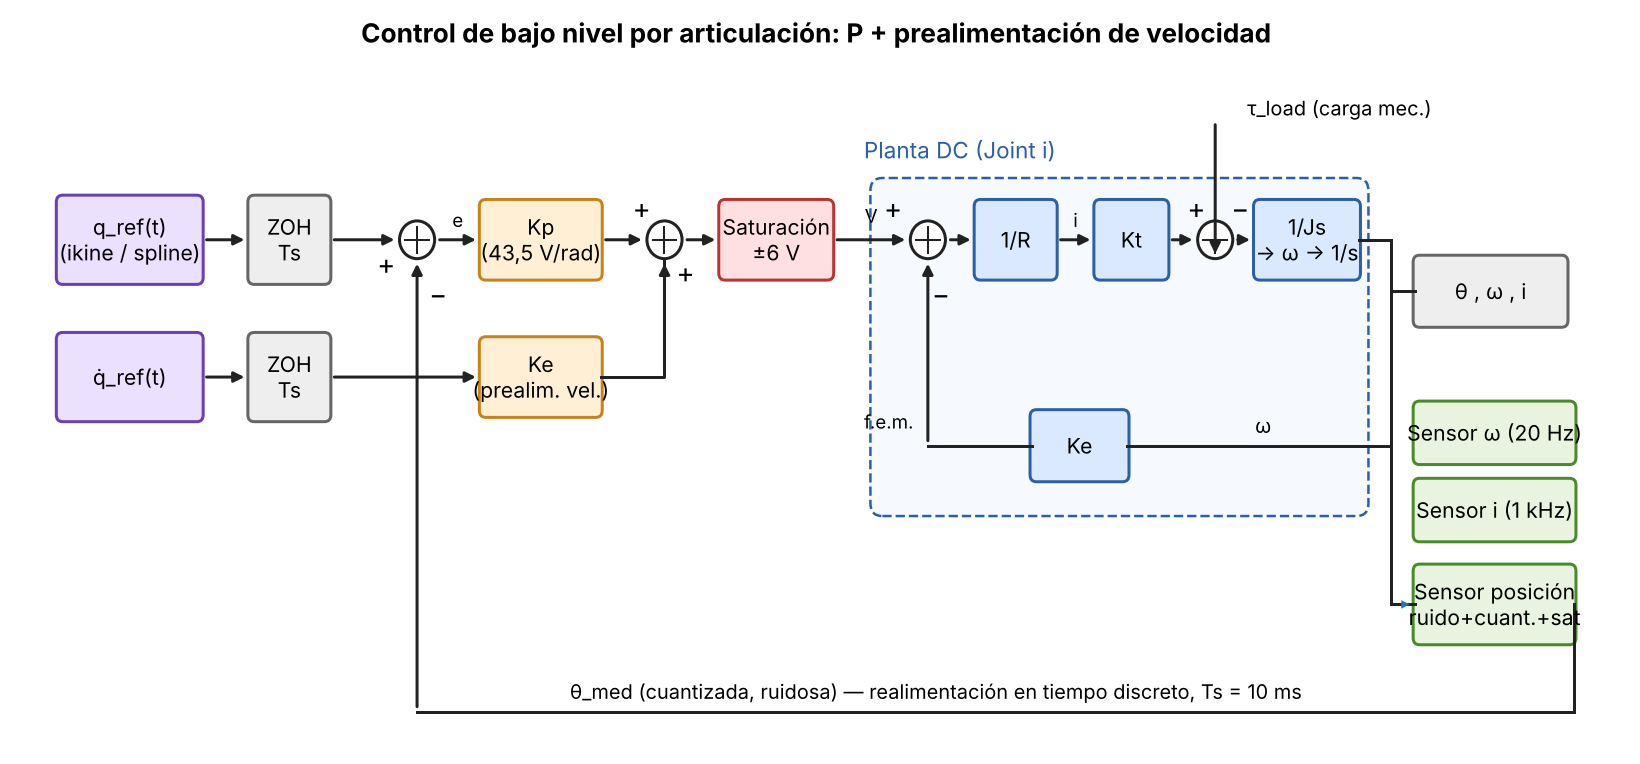
\includegraphics[width=\textwidth]{figuras/diag_lazo_bajo_nivel.png}
\caption{Lazo de bajo nivel por articulación: control P + prealimentación, planta DC y sensores.}\label{fig:lazo}\end{figure}
